\chapter{Visual Localization}

As stated in~\fullref{intro}, visual localization is the task of finding
the position of a camera that took a query photo relative to a reference scene
representation, and it is one of the fundamental problems in computer vision.

Compared to network-based localization methods, such as GNSS, visual localization,
even though being able to work in network-denied environments, comes with its own
set of problems that any successful method must consider. For both outdoor and
indoor localization, to which the field is typically separated due to different
localization complexity, illumination changes throughout the day and artificial lighting
influence present in the environment's representation data pose one class of such problems.
Further, it must cope with transient dynamic objects that can be present in both query
and database data, possibly occluding important feature-rich areas but having nothing
to do with the long-term visual appearance of the given location. Outdoors, seasonal and
weather-caused changes must be handled as well. For indoors, more problems stem from
textureless areas such as walls, ceilings, and floors; from repetition and symmetry
on both the global level with corridors, for example, and the local level, such as door handles.
Also, compared to outside, with typically longer distances between objects, inside small change
of viewing position leads to a vastly different view.

\section{Related work}

There are three main method categories for visual localization, as of \citet{torsten2018},
\citet{torsten2019}, \citet{torsten2021}, \citet{naverlabs}: methods based on structure,
image retrieval, and pose regression.

\subsubsection*{Structure-based methods}

Structure-based methods are the traditional way of estimating poses where a 3D model (the \emph{structure}) is
pre-created in order to later find 2D-3D correspondences.

% used https://arxiv.org/pdf/2007.13867.pdf
The 3D model is typically created by
Structure-from-Motion~\citep{SfM, schoenberger2016mvs}, by computing local sparse features (keypoints with descriptors,
\citet{LoweLocalization} used SIFT~\citep{SIFT} descriptor, \citet{PreSIFT} was pre-SIFT, using image rectification)
per database image with known focal length, match them against each other across images, and triangulate resulting 3D points
from these matches. Since the model already contains pre-computed features, matching against
a query image's features can then be performed. Since the 2D-3D matches are determined, the camera pose
is computed using the perspective-n-point (PNP) solver~\citep{PnP}. Because of the possible presence of outlier matches,
a RANSAC loop~\citep{RANSAC} is utilized to increase robustness. Other examples of this approach are~\citet{2D3D, 2D3D_2}.

With the growing size of a 3D point cloud, the runtime gets prolonged. To mitigate matching speed deterioration,
these methods also get paired with image retrieval, described next, to find the most
relevant images from the SFM model. Examples of these methods
are~\citet{InLoc, InLocRevisited, MegLoc}.

\subsubsection*{Image retrieval-based methods}

Image retrieval can be used to speed up the structure-based method family and make mapping
and localization more robust. That is because the restriction of matching to the parts of the scene visible in the given query photo
helps to avoid global ambiguities in the scene, e.g., caused by similar structures found in unrelated parts
of a scene~\citep{InLocRevisited}. It can also be used on its own for a closely related task to visual
localization called place recognition, which strives to find the approximate location of a query photo within a database
of geo-tagged images. Unlike visual localization, place recognition
does not need an explicit model representation, so no depth values nor point clouds are necessary for these
methods to work. Because of less input information, the location obtained by the retrieval and interpolating of several geo-tags
or camera poses is, in general, less accurate~\citep{InterpolationRetrieval, RegressionPose}.

In both cases, the goal is to gather a set of images that are the most similar according to a selected
criterion---here, a retrieved image is considered relevant if it sees the same scene---followed by an
optional re-ranking step. Historically, image retrieval methods have used variants of Bag of Visual Words~\citep{BoVW}
and Vector of Locally Aggregated Descriptors (VLAD)~\citep{VLAD},
newer approaches utilize features extracted by a Deep Neural Network (DNN) as such features encode high-level semantics
better than sparse features such as SIFT~\citep{RetrievalEE, DNNRegression, hausler2021patchnetvlad}.

\subsubsection*{Pose regression-based methods}

This category of methods uses a DNN for regressing the query pose end-to-end from an RGB image
directly to a 6~DoF pose. Based on the assumption that features obtained by a Neural Network (NN) trained for a general vision task
also include helpful information for pose estimation, transfer learning is leveraged for pose regression.

% https://arxiv.org/pdf/2207.05530.pdf
PoseNet~\citep{PoseNet} is an example of such an approach using an image classification CNN architecture, like
VGGNet or ResNet, with fully connected layers to regress the pose at the end of the architecture. Regression-based
methods are generally less accurate than structure-based localization (for PoseNet, by order of magnitude).
However, their advantage lies in short, constant inference time and smaller memory and computation power requirements
using just a single forward pass, even without requiring the camera intrinsics parameters, which may be
inaccurate and unavailable~\citep{RegressionAutoEnc}. The accuracy problem is inherent here, as end-to-end
learning imposes a tight coupling with the database coordinates. Thus, such a network can be seen as a compressed
version of the database itself, which limits the generalization power of the network~\citep{naverlabs}. As the approach is still
interesting for other use cases, many improvements were presented, such as~\citet{DNNRegression, Maps, VLocNet}
and~\citet{VLocNetpp}.


\section{InLoc}\label{sec:inloc}
This visual localization method, so-called \emph{Indoor Visual Localization with Dense Matching
and View Synthesis}, falls amid two-staged structure-based approaches combined with image retrieval. The first stage finds correspondences between a query image features and model of a scene, and the second estimates the camera pose.
The method's input is a database of RGBD
images with known focal lengths (from EXIF data, for instance), and the method internally uses a point cloud 3D scene
representation. The method focuses on indoor localization and addresses several 
issues presented in~\fullref{intro}. Visual representation of the method with a short summary can be seen in~\cref{fig:inloc_intro}. 

\begin{figure}
    \centering
    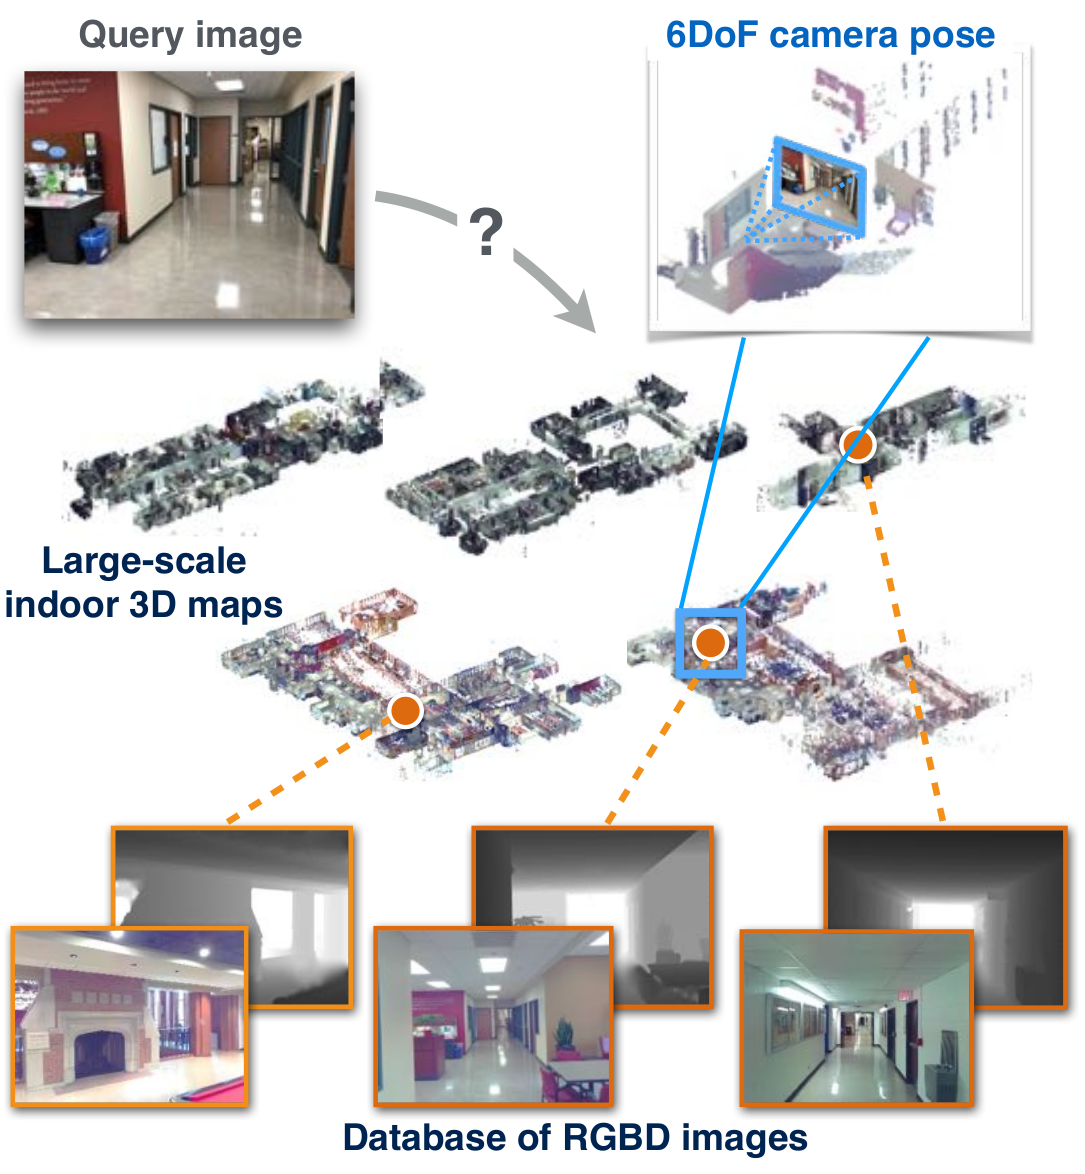
\includegraphics[width=.5\textwidth]{../graphics/inloc.png}
    \caption{Given a database of geometrically-registered RGBD images, InLoc predicts
    the 6~DoF camera pose of a query RGB image by retrieving candidate images, estimating candidate camera poses, and selecting
    the best matching camera pose. Image taken from~\citet{InLoc}.}\label{fig:inloc_intro}
\end{figure}

All of illumination changes~(1), textureless areas~(3) leading to lack of sparse local features, such as SIFT~\citep{SIFT},
repetitive elements in indoor settings~(4) leading to similar repetitive features being produced, and even viewpoint changes~(5)
are overcome by utilizing multi-scale dense CNN features computed densely on a regular grid by NetVLAD~\citep{NetVLAD}.
These features are used for database image retrieval, as $N=100$ best matching images are chosen based on sorted
normalized L2 distances of the extracted database feature vectors and the query feature vector.

In the next stage, candidate images are re-ranked by another feature matching in the geometric verification process and
pose estimation. Firstly, features are extracted by VGG~\citep{VGG16} model on conv5 and subsequently on conv3 layer
restricted by previously found matches are used for finding geometrically consistent sets of correspondences with
RANSAC~\citep{RANSAC}. Based on the number of RANSAC inliers, top $M = 10$ candidate database images are kept.
It is to be noted that these features are obtained with no additional computation burden as VGG is used internally
by NetVLAD. As database images used as input to the method are RGBD and hence they have associated 3D points, the
query camera pose is then estimated by finding pixel-to-pixel correspondences between the query and the top
$M$~database images followed by P3P-LO-RANSAC~\citep{P3PLORANSAC}.

To further cope with self-similarity found in indoor locations, counting the number of inliers
as positive evidence to decide whether two views are taken from an exact location is not the
only decisive criterion. Negative evidence is also used in the form of the portion of the view
rendered from the candidate query pose that does not match the query photo. Authors of the paper
refer to this as \emph{explicit pose estimate verification based on view synthesis}. Verification
is done pixel-wise to obtain consistent and inconsistent pixels between the render and the query photo.
To keep invariance to illumination changes and small misalignments, pixel comparison operates with RootSIFT
local patch descriptors~\citep{RootSIFT}. The final image-render similarity is the median of descriptor distance
across the entire image while ignoring areas with missing 3D structure resulting in background-filled regions in renders.

This thesis further examines the view synthesis part of the verification process as it changes the rendered source imputed
to the RootSIFT descriptor computation process. In further chapters, three rendering
techniques alternative to the initial article's rendering process are described in detail.

The decision to use the InLoc method in the thesis was driven by the fact that it is the first method of its kind,
state-of-the-art of its time that puts basis or plays a role of a baseline for
other subsequent state-of-the-art methods~\citep{PoseCorrection}. Further, its source codes are publicly
available\footnotei{,}{http://www.ok.sc.e.titech.ac.jp/INLOC/} whereas a subsequent paper~\citep{InLocRevisited}
presenting some improvements does not provide source codes.
